\newchapter{Validierung}
\label{kap:6}


In diesem Kapitel wollen wir numerische Beispiele für das Hindernis- bzw. Kontaktproblem diskutieren. Dabei werden Auswertungen verwendet, die aus dem Quellcode aus Anhang \ref{anhang:D} resultieren.

Die untersuchten numerischen Beispiele wurden aus den Veröffentlichun-gen \cite{SiebVee}, \cite{BraeCar}, \cite{BraeCar2} und \cite{CarWri} entnommen.


\section{Numerische Beispiele zum Hindernisproblem}
\label{kap:6.1}

\begin{bsp}[glatte, rotationssymmetrische Lösung]\label{bsp:6.1}
Wir betrachten das Hindernisproblem mit dem Hindernis $\psi \equiv 0$ und der Lastfunktion $f\equiv -2$ auf $\Omega = [-\frac 32,\frac 32]^2$. Die Dirichlet-Randbedingungen\index{Randbedingungen!Dirichlet} werden durch die Funktion
\[
	\tilde u(x,y) = \frac{x^2+y^2}2-\frac 12 \ln(x^2+y^2)-\frac 12
\]
gegeben. Für dieses Problem existiert eine exakte (glatte) Lösung, die in \idx{Polarkoordinaten} wie folgt lautet:
\begin{align}\label{eq:6.1}
	u(r,\varphi) = \begin{cases}
					\frac{r^2}2-\ln (r)-\frac 12 & , r \ge 1 \\
					0 & , \, \text{sonst}
				\end{cases} \, .
\end{align}
Damit lässt sich der exakte Wert des Energiefunktionals $J(u)$ mit \eqref{eq:6.1} ermitteln. Hierfür nutzen wir die Rotationssymmetrie von $u$ aus, da $u$ unabhängig vom Drehwinkel $\varphi$ ist. Dadurch reicht es aus, die zu berechnenden Integrale nur im ersten Quadranten von $\Omega$ zu berechnen. Um jetzt $J(u)= \frac 12 a(u,u)-(f,u)$ zu bestimmen, müssen wir mit der Kettenregel den Zusammenhang zwischen $u_x,u_y$ und $u_r,u_\varphi$ ermitteln. Dieser ergibt sich zu
\begin{align}\label{eq:6.2}
	\begin{pmatrix} u_x \\ u_y \end{pmatrix} = \frac 1r \begin{pmatrix} r \cos \varphi & -\sin\varphi \\ r \sin\varphi & \cos\varphi \end{pmatrix} \begin{pmatrix} u_r \\ r_\varphi \end{pmatrix}.
\end{align}

Da $u_\varphi = 0$ und $u_r = r-\frac 1r$ gilt, erhalten wir für den exakten Wert des Energiefunktionals unter Verwendung von \eqref{eq:6.2}
\begin{align*}
	J(u) & = \frac 12 \int_\Omega \underbrace{\nabla u \nabla u}_{=u_x^2+u_y^2} \, dx dy - \int_\Omega f u \, dx dy \\
	& = 4  \( \frac 12 \int_0^{\frac \pi4} \int_1^{\frac 3{2\cos\varphi}} (\cos^2\varphi + \sin^2\varphi) \(r-\frac 1r\)^2 r \, dr d\varphi  \right. \\
	& \quad + \frac 12 \int_{\frac \pi4}^{\frac {3\pi}4} \int_1^{\frac 3{2\sin\varphi}} (\cos^2\varphi + \sin^2\varphi) \(r-\frac 1r\)^2 r \, dr d\varphi \\
	&\quad  +  2 \int_0^{\frac \pi4} \int_1^{\frac 3{2\cos\varphi}} \(\frac{r^2}2 - \ln(r) - \frac 12\) r \, dr d\varphi  \\
	&\quad  + \left. 2 \int_{\frac \pi4}^{\frac {3\pi}4} \int_1^{\frac 3{2\sin\varphi}} \(\frac{r^2}2 - \ln(r) - \frac 12\) r \, dr d\varphi \) \\
	& \approx 3,980995748730258 \, .
\end{align*}
Die oberen Grenzen $\frac 3{2\cos\varphi}$ und $\frac 3{2\sin\varphi}$ kommen dabei durch Beschreibung der Randpunkte von $\Omega$ in Polarkoordinaten für $\varphi\in [0,\frac\pi4]$  zustande. Die Rotationssymmetrie kann auf das zweite Integral nur deshalb angewendet werden, weil $f$ eine konstante (und damit auch rotationssymmetrische) Funktion ist.


\begin{figure}[h]
\begin{center}
\subfigure[Exakte Lösung für das Hindernisproblem]{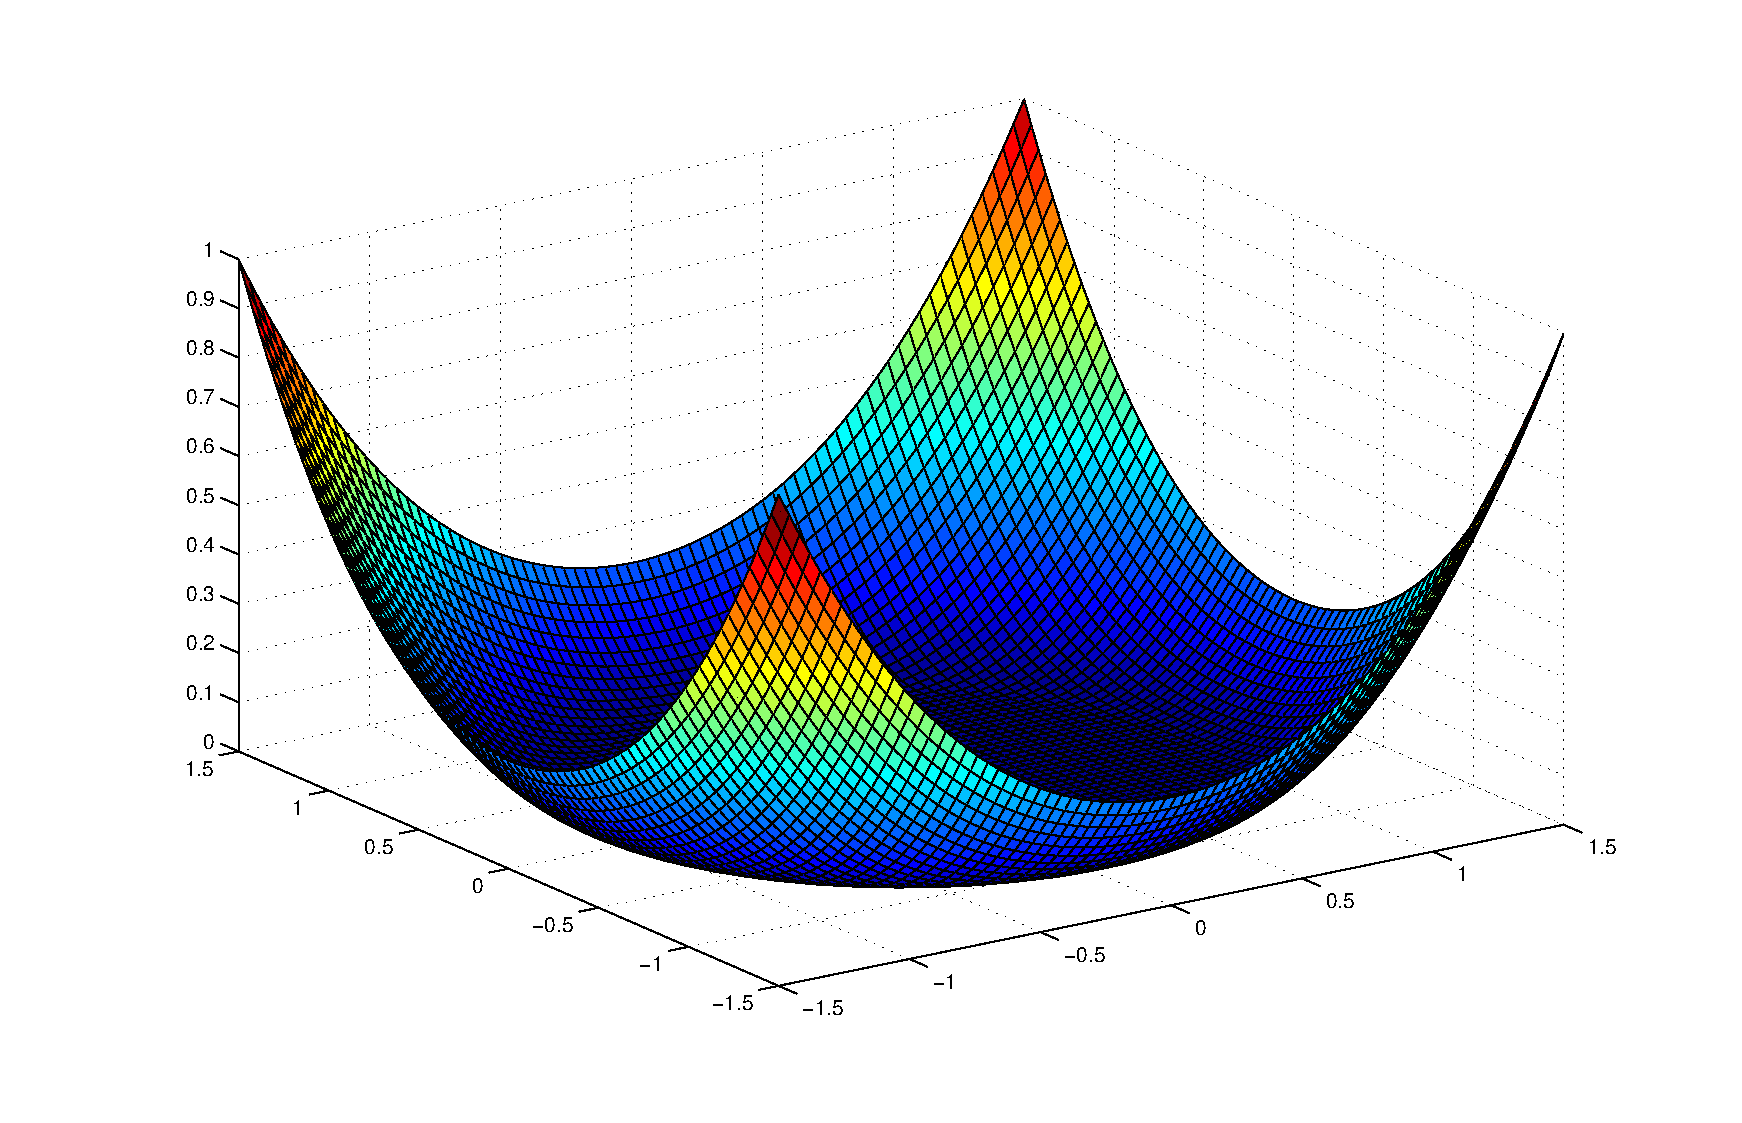
\includegraphics[width=6.25cm]{Abbildungen/exakte_loesung_hindernisproblem1.eps}}
\hfill
\subfigure[Numerische Lösung in der Verfeinerungsstufe 6 mit $\theta_1=0,4$ und $\theta_2=0,3$]{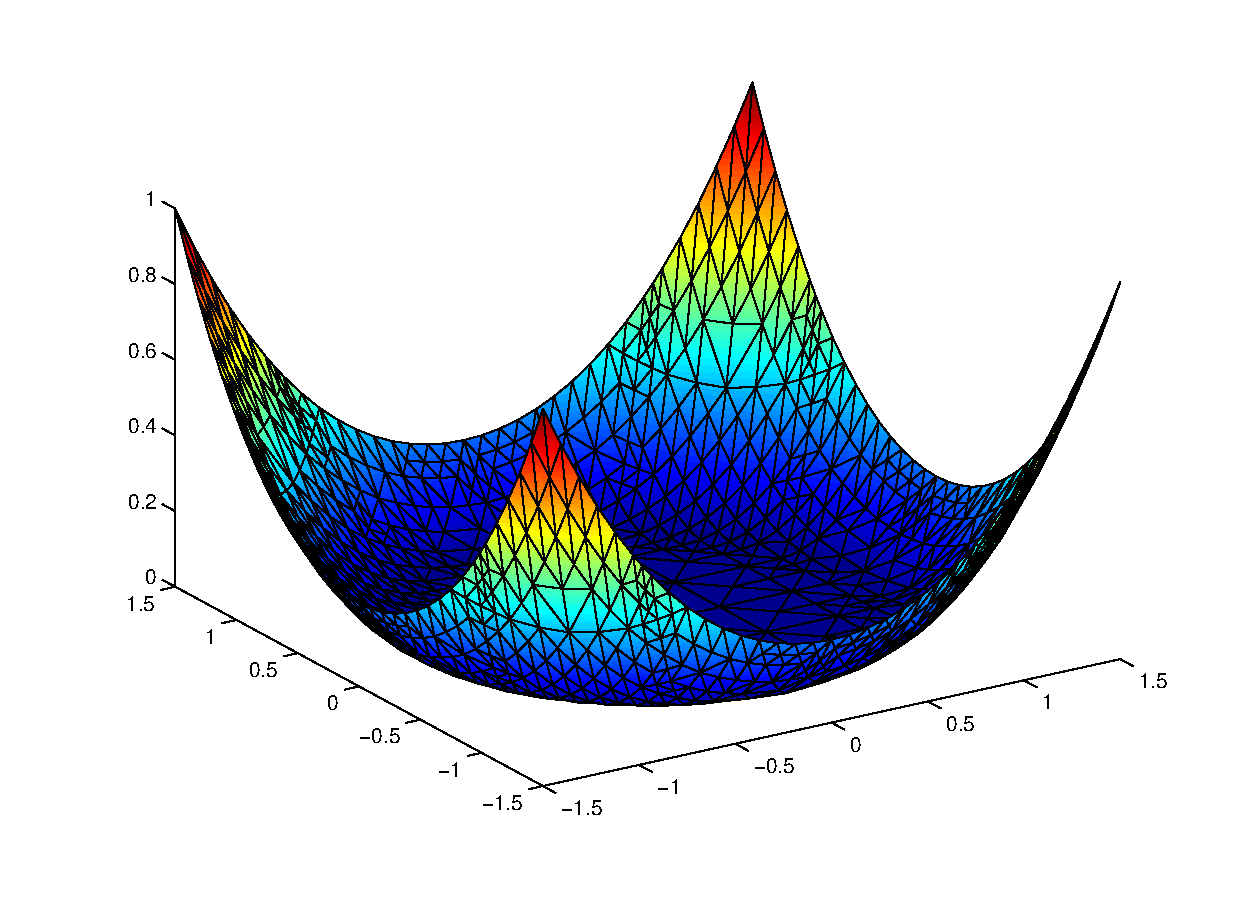
\includegraphics[width=6.25cm]{Abbildungen/num_loesung_bsp1_rec6_0,6_0,5.eps}}
\end{center}
\caption{Exakte und numerische Lösung des Beispiels \ref{bsp:6.1}\label{abb:6.1}}
\end{figure}


\begin{figure}[h]
\begin{center}
\subfigure[Verfeinerungsstufe 6]{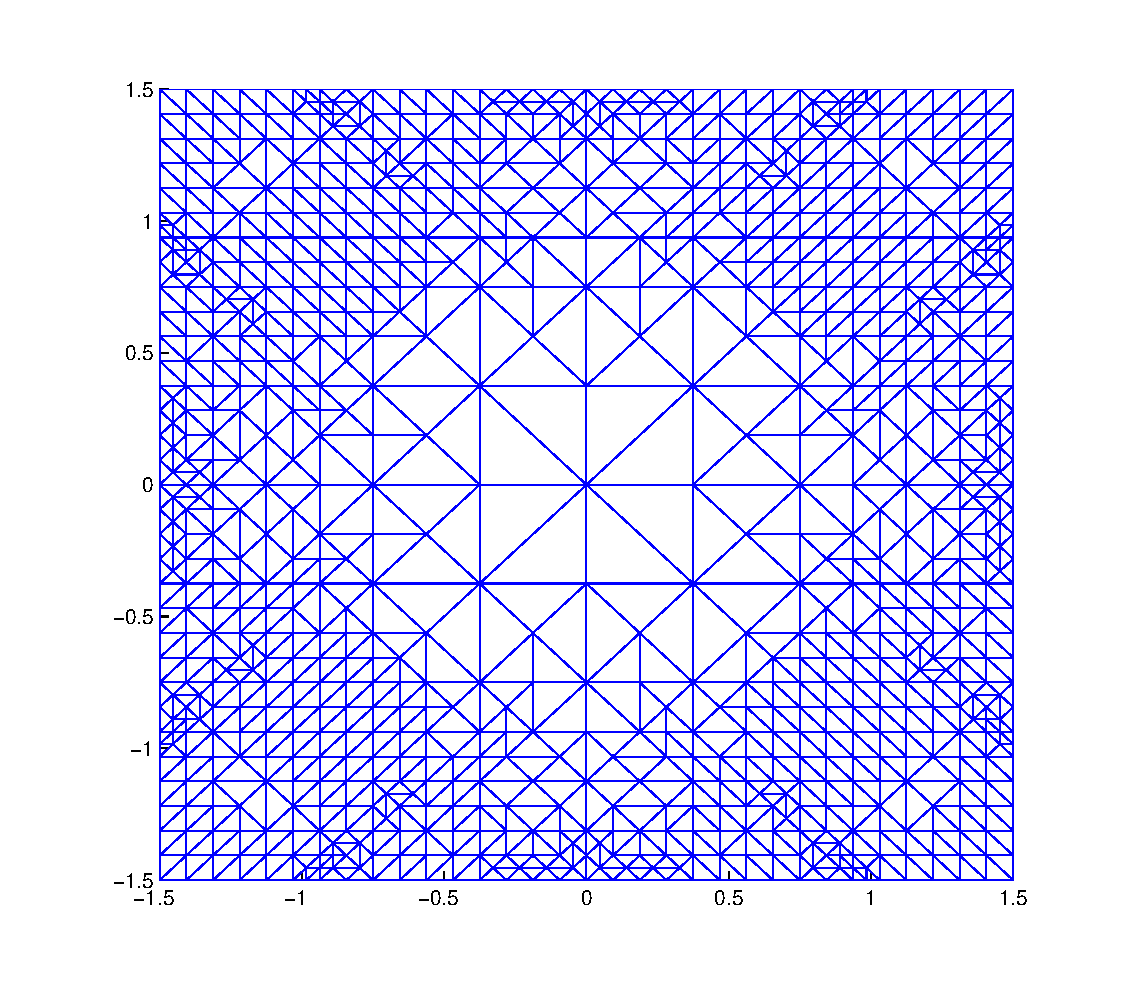
\includegraphics[width=6.2cm]{Abbildungen/mesh_rec6_bsp1.eps}}
\hfill
\subfigure[Verfeinerungsstufe 8]{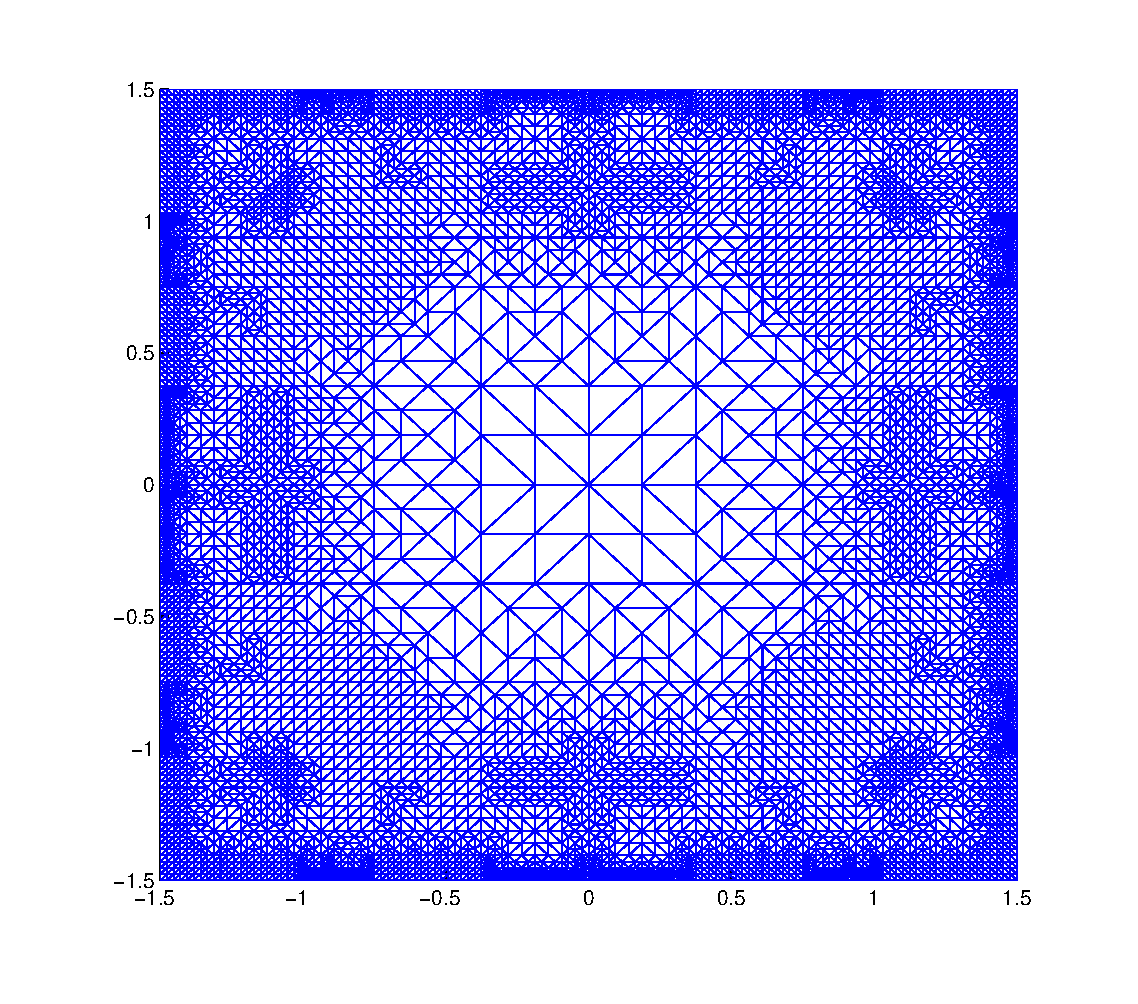
\includegraphics[width=6.25cm]{Abbildungen/mesh_rec8_bsp1.eps}}
\end{center}
\caption{Gitterverfeinerung für das Hindernisproblem im Beispiel \ref{bsp:6.1} mit $\theta_1=0,4$ und $\theta_2=0,3$\label{abb:6.2}}
\end{figure}

In Abbildung \ref{abb:6.1} ist die exakte Lösung und die Galerkin-Lösung auf der Verfeinerungsstufe 6 der implementierten, adaptiven Verfeinerungsstrategie im Vergleich dargestellt. In der Tabelle \ref{tab:6.1} sind die Ergebnisse für das Beispiel für $\theta_1 = 0,3$ und $\theta_2 = 0,2$, sowie für eine uniforme Verfeinerung angegeben. Die maximale Anzahl der Knoten $\abs{\mcal N}$ ist jeweils mittels der Implementierung auf 150.000 begrenzt. Man kann gut erkennen, dass die Anzahl der Knoten im uniformen Fall wesentlich schneller ansteigt. Da in den ersten Verfeinerungsstufen sehr wenig Knoten vorhanden sind, gleichen sich zunächst die adaptive und uniforme Verfeinerung. Der starke Anstieg des Freiheitsgrades in den letzten beiden Schritten liegt daran, dass die lokalen Anteile des Fehlerindikators $\rho_{\mcal S}$ sehr klein werden (wegen hoher Knotenanzahl) und kann durch eine variable Wahl der Parameter $\theta_1$ und $\theta_2$ verringert werden. 

Weiter stellen wir in Abbildung \ref{abb:6.2} eine adaptive Gitterverfeinerung für das Beispiel \ref{bsp:6.1}, das mit {\ttfamily start_example_1.m} für $\theta_1 = 0,4$ und $\theta_2 = 0,3$ erzeugt werden kann, in den Stufen 6 und 8 dar und man kann gut erkennen, dass im Bereich des vollen Kontaktes weniger stark verfeinert wird. Weiter kann man sehen, dass durch die Option {\ttfamily 'symmetric'} das Gitter auch symmetrisch  von Verfeinerungsschritt zu Verfeinerungsschritt angeordnet bleibt.


\begin{table}[h]
\centering
\begin{tabular}[c]{|c|c|c|c|c|c|c|c|}
	\hline
	 & \multicolumn{4}{c|}{Adaptive Verfeinerung} & \multicolumn{2}{c|}{Uniforme Verfeinerung} \\
	\hline
	Stufe & $\abs{\mcal N}$ & $\rho_{\mcal S}(\eps_{\mcal V})$ & $-\mcal I_{\mcal Q} (\eps_{\mcal V})$ & $-\mcal I(e)$ & $\abs{\mcal N}$ & $-\mcal I (e)$ \\
	\hline
	 1 &  9  & 6.3512 & 3.1756 & 4.6323 & 9  & 4.6323 \\
	 2 & 25 & 1.8284 & 0.9142 & 1.0978 & 25 & 1.0978 \\
	 3 & 81 & 0.8642 & 0.4349 & 0.2667 & 81 & 0.2667 \\
	 4 & 197 & 0.5422 &0.2713 & 0.1113 & 289 & 0.0670 \\
	 5 & 357 & 0.3896 & 0.1949 & 0.0564 & 1089 &0.0167  \\
	 6 & 821 & 0.2564 & 0.1282 & 0.0231 &4225 &  0.0046 \\
	 7 & 1133 & 0.1896 & 0.0948 & 0.0141 & 16641 & 0.0014 \\
	 8 & 1957 & 0.0993 & 0.0497 & 0.0079 & 66049 & 0.0010 \\
	 9 & 7569 & 0.0476 & 0.0238 & 0.0020 & & \\
	 10 & 29761 & 0.0223 & 0.0112 & 0.0018 & & \\
	 11 & 118017 & 0.0075 & 0.0037 & 0.0007 & & \\
	\hline
\end{tabular}
\caption[Vergleich von adaptiver und uniformer Verfeinerung für Beispiel \ref{bsp:6.1}]{\label{tab:6.1}Vergleich von adaptiver ($\theta_1 = 0,4;\theta_2 = 0,3$) und uniformer Verfeinerung für Beispiel \ref{bsp:6.1} mit Angabe des Freiheitsgrades, a posteriori Fehlerschätzer und exaktem Fehler}
\end{table}


In Abbildung \ref{abb:6.3} sind die Oszillationen in für mehrere Verfeinerungsstufen $k$ dargestellt. Dabei kann man erkennen, dass es in der Stufe $k=1$ noch einen isolierten Knoten, den Ursprung, gibt, der jedoch durch Verfeinerung verschwindet, weil es keinen äquivalenten, isolierten Kontaktpunkt für die exakte Lösung gibt. Außerdem können wir sehen, dass durch die Bedingung aus Lemma \ref{lem:4.24} der Wert der Oszillationsterme von Verfeinerung zu Verfeinerung sinkt.



\begin{figure}[h]
\begin{center}
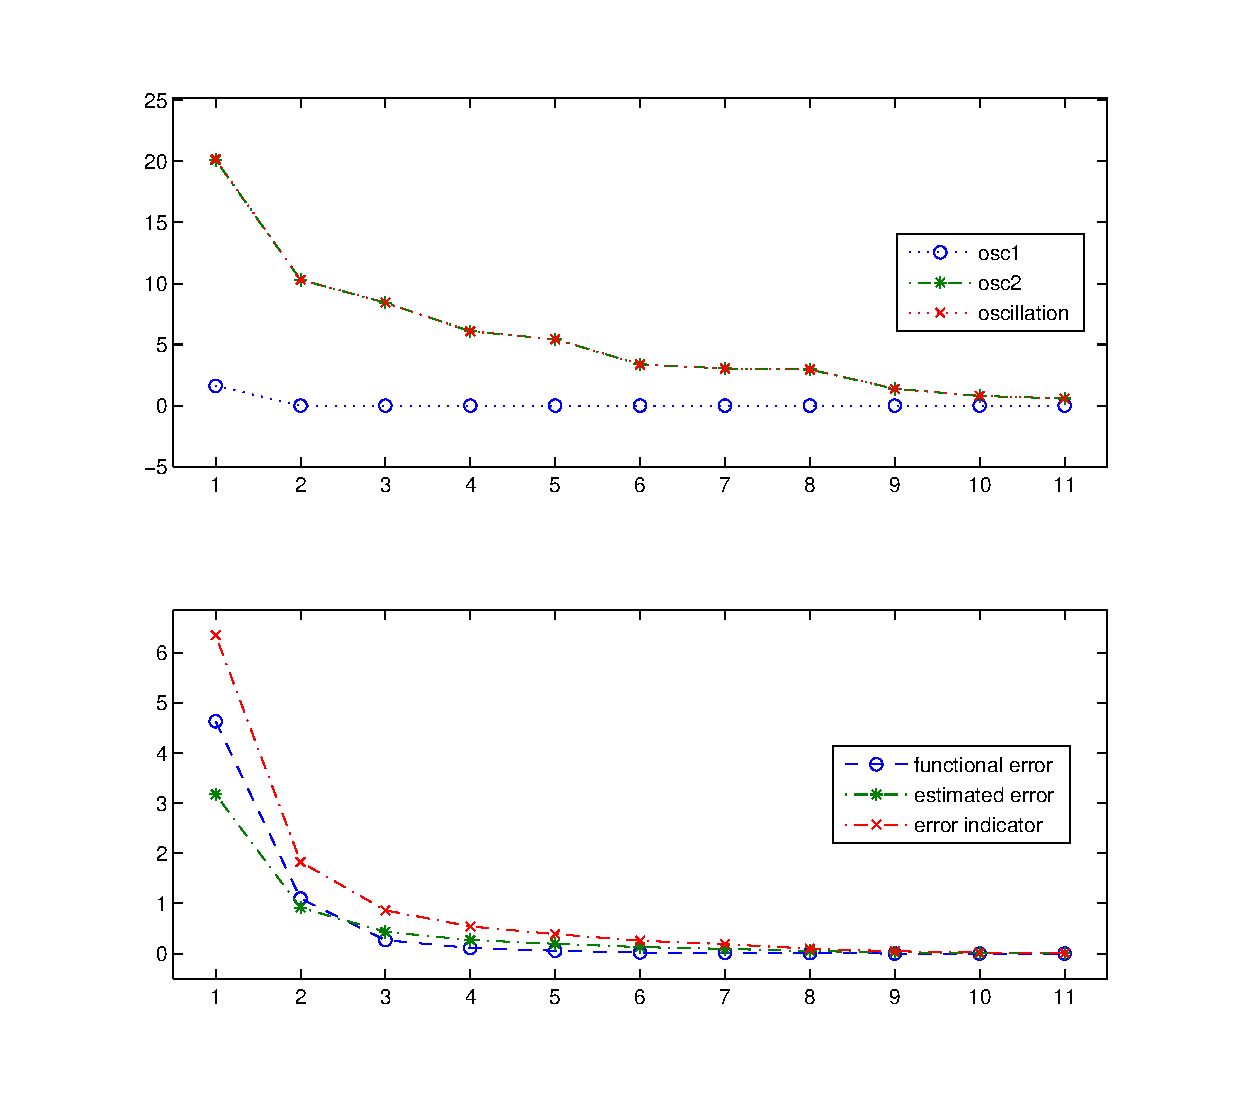
\includegraphics[width=10.5cm]{Abbildungen/adaptive_solution_example1.ps}
\end{center}
\caption[Diagramm mit dem Fehler und der Oszillation für Beispiel \ref{bsp:6.1}]{Oszillationsterme, Fehlerindikator $\rho_{\mcal S}$, Fehlerschätzer $-\mcal I_{\mcal Q}$ und exakten Fehler für Beispiel \ref{bsp:6.1} mit $\theta_1=0,3$ und $\theta_2=0,2$\label{abb:6.3}}
\end{figure}
\end{bsp}


\newpage


\begin{bsp}[Singularität und L-förmiges Gebiet]\label{bsp:6.2}
Wir wollen nun ein Hindernisproblem mit Singularität im Nullpunkt betrachten, was zu einer starken Verfeinerung an diesem Punkt führen muss. Hierfür sei das Gebiet L-förmig, also von der Form
\[
	\Omega \coloneqq (-2,2)^2 \setminus ([0,2]\times [-2,0]) \, .
\]
Das Hindernis sei wieder durch $\psi \equiv 0$ gegeben und die Lastfunktion in Polarkoordinaten $(r,\varphi)$ durch
\[
	f(r,\varphi) \coloneqq -r^{\frac 23} \sin \(\frac{2\varphi}3\)\(\frac{\gamma_1'(r)}r + \gamma_1''(r)\) - \frac 43r^{\frac 13} \gamma_1'(r) \sin \(\frac{2\varphi}3\)-\gamma_2(r) \, ,
\]
wobei mit $\bar r = 2\(r-\frac 14\)$ gilt
\begin{align*}
	\gamma_1(r) &= \begin{cases}
					1 & , \bar r < 0 \\
					-6\bar r^5+15 \bar r ^4-10 \bar r ^3+1 & , 0 \le \bar r < 1 \\
					0 & , \bar r \ge 1
				\end{cases} \, , \\
	\gamma_2(r) & = \begin{cases}
						0 & , r < \frac 5 4 \\
						1 & , \, \text{sonst}
					\end{cases} \, .
\end{align*}
Für dieses Problem gibt es eine exakte Lösung, die in Polarkoordinaten
\[
	u(r,\varphi) = r^{\frac 23} \gamma_1(r)\sin \(\frac{2\varphi}3\) 
\]
lautet. Die Funktion hat im Ursprung eine Singularität. Damit können wir auch für dieses Beispiel mit den Umformungen aus \eqref{eq:6.2} den exakten Wert des Energiefunktionals $J$ berechnen. Durch Anwendung der Polarkoordinaten und Transformationssatz der Integration erhalten wir
\[
	J(u) \approx 0,5 \, .
\]

\begin{table}[h]
\centering
\begin{tabular}[c]{|c|c|c|c|c|c|c|c|}
	\hline
	 & \multicolumn{4}{c|}{Adaptive Verfeinerung} & \multicolumn{2}{c|}{Uniforme Verfeinerung} \\
	\hline
	Stufe & $\abs{\mcal N}$ & $\rho_{\mcal S}(\eps_{\mcal V})$ & $-\mcal I_{\mcal Q} (\eps_{\mcal V})$ & $-\mcal I(e)$ & $\abs{\mcal N}$ & $-\mcal I (e)$ \\
	\hline
	 1 &  65  & 0.3926 & 0.1963 & 4.6323 & 65 & 0.4288 \\
	 2 & 83 & 0.3081 & 0.1560 & 1.0978 & 225 & 0.2164 \\
	 3 & 134 & 0.1777 & 0.0894 & 0.2667 & 833 & 0.0669  \\
	 4 & 215 & 0.1136 &0.2713 & 0.0572 & 3201 & 0.0242 \\
	 5 & 332 & 0.0704 & 0.1949 & 0.0355 & 12545 & 0.0183 \\
	 6 & 503 & 0.0469 & 0.1282 & 0.0235 & 49665 & 0.0078 \\
	 7 & 1315 & 0.0169 & 0.0948 & 0.0085 & 197633 & ––––––  \\
	 8 & 5181 & 0.0074 & 0.0497 & 0.0039 &  &  \\
	 9 & 20569 & 0.0051 & 0.0238 & 0.0020 & & \\
	 10 & 81968 & 0.0034 & 0.0112 & 0.0013 & & \\
	\hline
\end{tabular}
\caption[Vergleich von adaptiver und uniformer Verfeinerung für Beispiel \ref{bsp:6.2}]{\label{tab:6.2}Vergleich von adaptiver ($\theta_1 = \theta_2 = 0,3$) und uniformer Verfeinerung für Beispiel \ref{bsp:6.2} mit Angabe des Freiheitsgrades, a posteriori Fehlerschätzer und exaktem Fehler}
\end{table}

In Tabelle \ref{tab:6.2} sind die Ergebnisse der adaptiven Verfeinerung des Problems mit den Parametern $\theta_1 = \theta_2=0,3$ dargestellt, die mit der Funktion {\ttfamily start_example_2.m} erzeugt werden können. Diese Ergebnisse sind auch in Abbildung \ref{abb:6.6} im Diagram dargestellt.

Die Abbildungen \ref{abb:6.4} und \ref{abb:6.5} zeigen die Lösung in der Verfeinerungsstufe 7 und zwei verfeinerte Gitter. Wir können daran erkennen, dass, wie erwartet, gerade um die Singularität im Ursprung eine starke Netzverfeinerung stattfindet. In diesem Bereich ist zudem kein Kontakt mit dem Hindernis vorhanden, was die adaptive Verfeinerung nochmals untermauert.

Insgesamt beschreiben die Ergebnisse grundlegend dasselbe Verhalten, wie wir schon in Beispiel \ref{bsp:6.1} erkennen konnten.

\begin{figure}[h]
\begin{center}
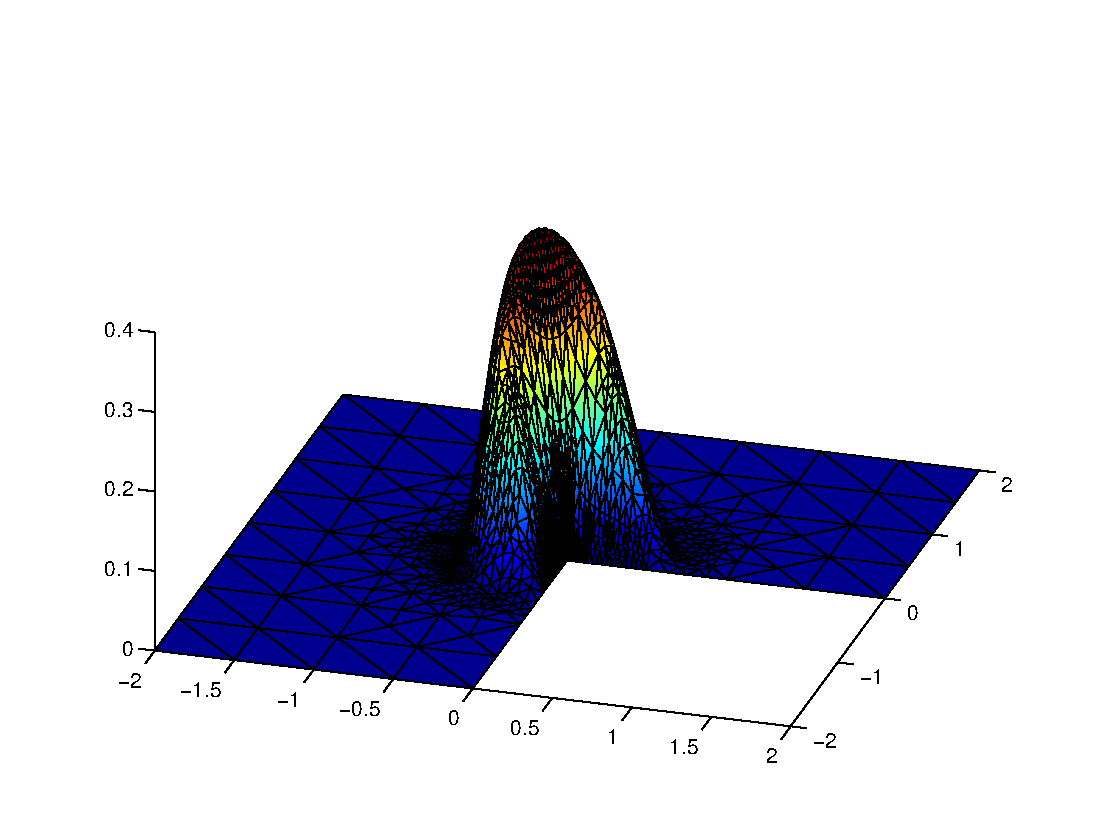
\includegraphics[width=13cm]{Abbildungen/num_loesung_rec7_bsp2.eps}
\end{center}
\caption{Numerische Lösung des Beispiels \ref{bsp:6.2} in der Verfeinerungsstufe 7 mit $\theta_1=\theta_2 = 0,3$\label{abb:6.4}}
\end{figure}

\begin{figure}[h]
\begin{center}
\subfigure[Verfeinerungsstufe 6]{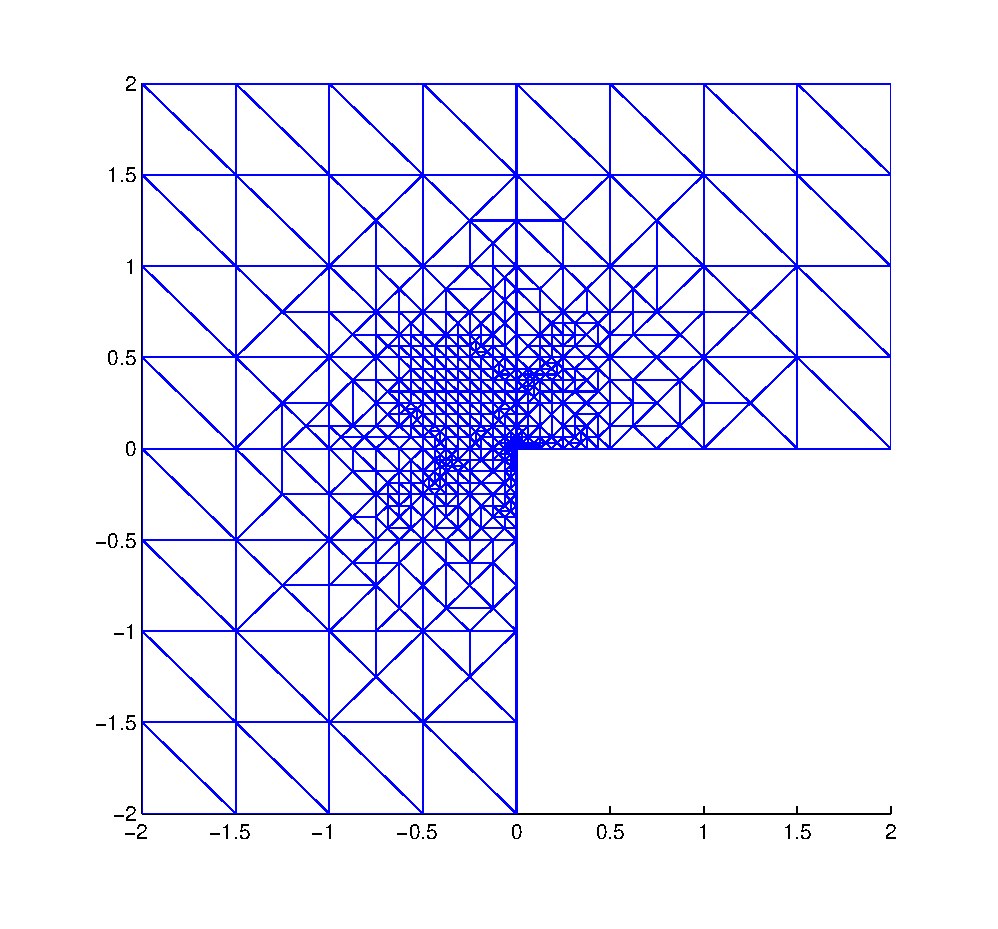
\includegraphics[width=6.26cm]{Abbildungen/mesh_rec6_bsp2.eps}}
\hfill
\subfigure[Verfeinerungsstufe 8]{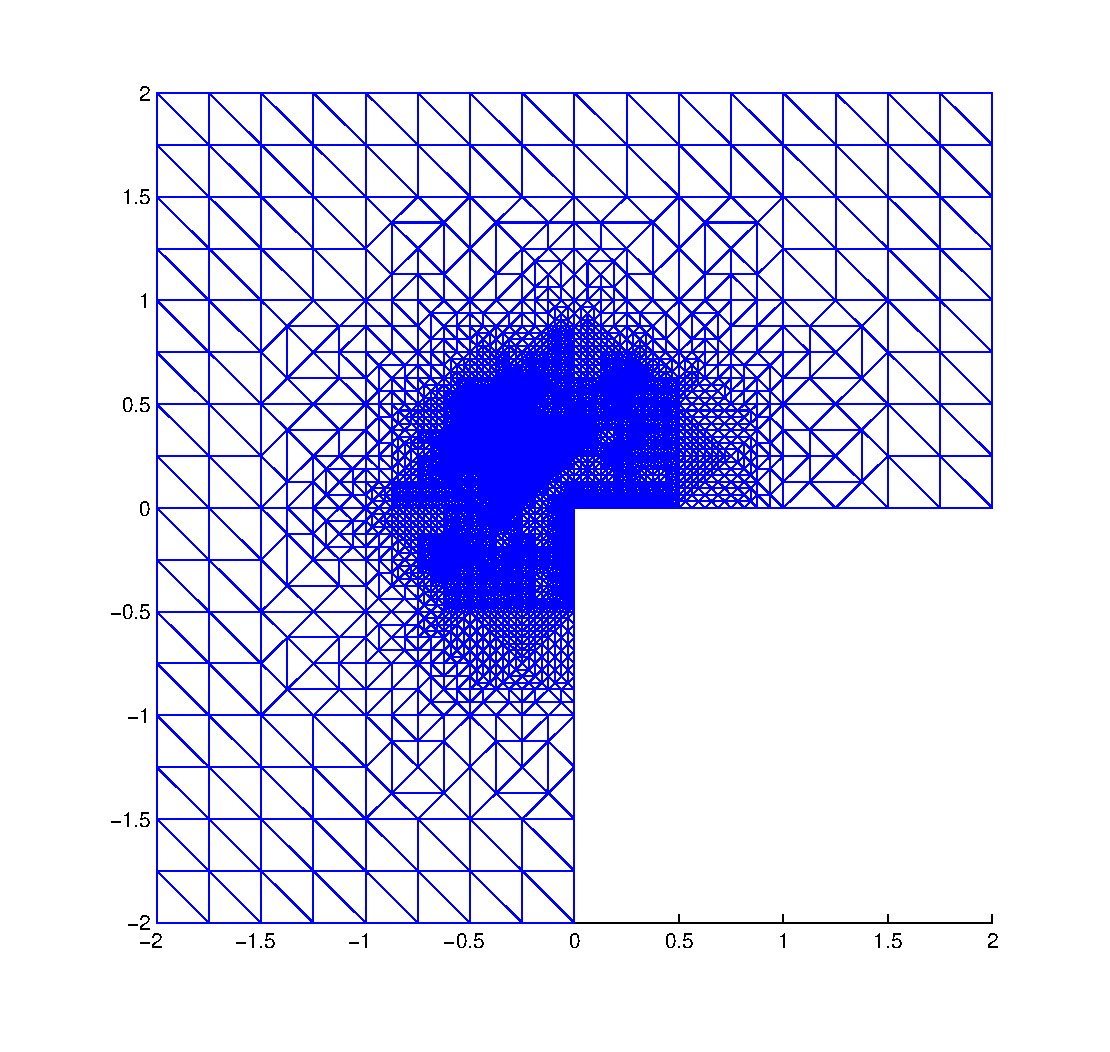
\includegraphics[width=6.26cm]{Abbildungen/mesh_rec8_bsp2.eps}}
\end{center}
\caption{Netzverfeinerungen für das Beispiel \ref{bsp:6.2} mit $\theta_1=\theta_2=0,3$\label{abb:6.5}}
\end{figure}

\begin{figure}[h]
\begin{center}
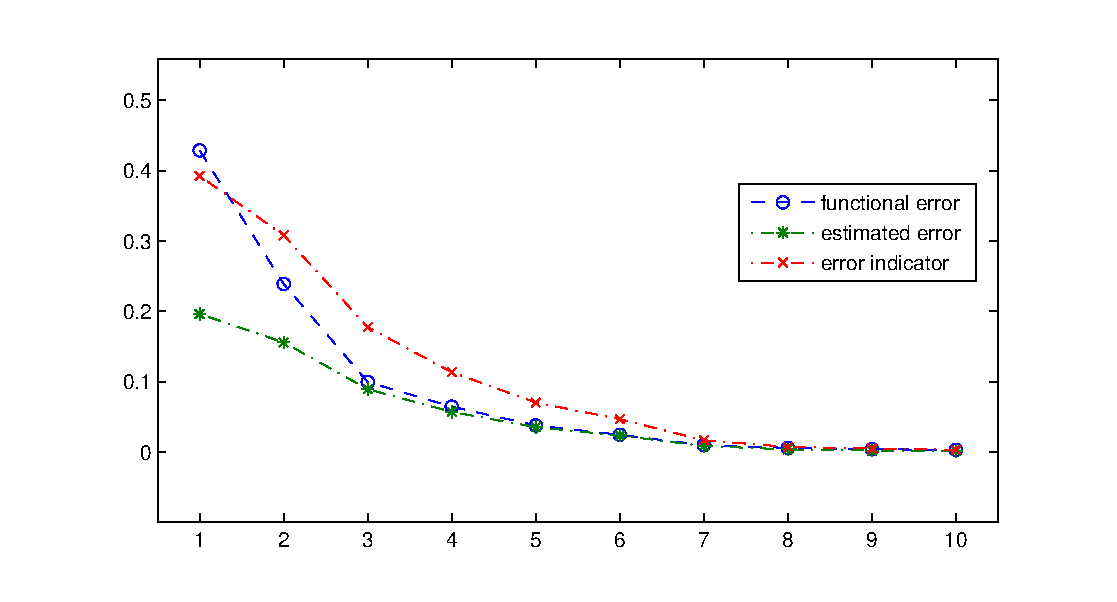
\includegraphics[width=11cm]{Abbildungen/adaptive_solution_example2.eps}
\end{center}
\caption[Diagramm mit dem Fehler und der Oszillation für Beispiel \ref{bsp:6.2}]{Fehlerindikator $\rho_{\mcal S}$, Fehlerschätzer $-\mcal I_{\mcal Q}$ und exakten Fehler $-\mcal I(e)$ für Beispiel \ref{bsp:6.2} mit $\theta_1=0,3$ und $\theta_2=0,3$\label{abb:6.6}}
\end{figure}
\end{bsp}

\clearpage

\begin{bsp}\label{bsp:6.3}
Als letztes Beispiel für ein affines Hindernisproblem können wir das Beispiel \ref{bsp:6.2} noch erweitern, indem wir als affines Hindernis nicht die Nullfunktion, sondern eine umgedrehte Pyramide verwenden, die gegeben wird durch
\[
	\psi (x) \coloneqq 0,5 \,  (\dist (x,\partial [-2,2]^2)-2,01) \, , \quad x \in \bar \Omega \, ,
\]
während alle übrigen Eingabedaten gleich bleiben. In Abbildung \ref{abb:6.7} können wir das Hindernis gut an der Ecke des Gebietes $\Omega$ erkennen, wenn wir diese mit der Lösung von Beispiel \ref{bsp:6.2} aus Abbildung \ref{abb:6.4} vergleichen.

Da für dieses Problem keine exakte Lösung bekannt ist, berechnen wir uns einen Referenzwert für den Wert $J(u)$, indem wir das Problem für ein engmaschiges Gitter ($h=0,05$) berechnen. Damit ergibt sich
\[
	J(u) \approx -0,8250\, .
\]

In den Abbildungen \ref{abb:6.7} und \ref{abb:6.8} sind wieder die Lösung und verschiedene Verfeinerungsstufen vom Gitter für das gegebene Problem mit den Parametern $\theta_1=\theta_2=0,3$ dargestellt, die mit der Datei {\ttfamily start_example_3.m} erzeugt werden können. Weiter sind in der Tabelle \ref{tab:6.3} die Daten aus dem Diagram der Abbildung \ref{abb:6.9} aufgeführt.

Auch in diesem Beispiel kann man die grundlegende Entwicklung des Fehlerschätzers bzw. Fehlers im Funktional gut erkennen. An den Verfeinerungsstufen kann man deutlich sehen, dass erneut am Ursprung  eine starke Verfeinerung stattfindet (s. die Singularität aus Beispiel \ref{bsp:6.2}) und zudem ist am Rand eine feinere Triangulierung zu erkennen. Dies kann daran liegen, dass hier  eine starke Veränderung in der Funktion (vgl. Abbildung \ref{abb:6.7}) vorliegt und daher viele Informationen verwertet werden müssen.


\begin{figure}[h]
\begin{center}
\includegraphics[width=13cm]{Abbildungen/num_loesung_bsp3.eps}
\end{center}
\caption{Numerische Lösung des Beispiels \ref{bsp:6.3} mit $\theta_1=\theta_2 = 0,3$\label{abb:6.7}}
\end{figure}


\begin{figure}[h]
\begin{center}
\subfigure[Verfeinerungsstufe 6]{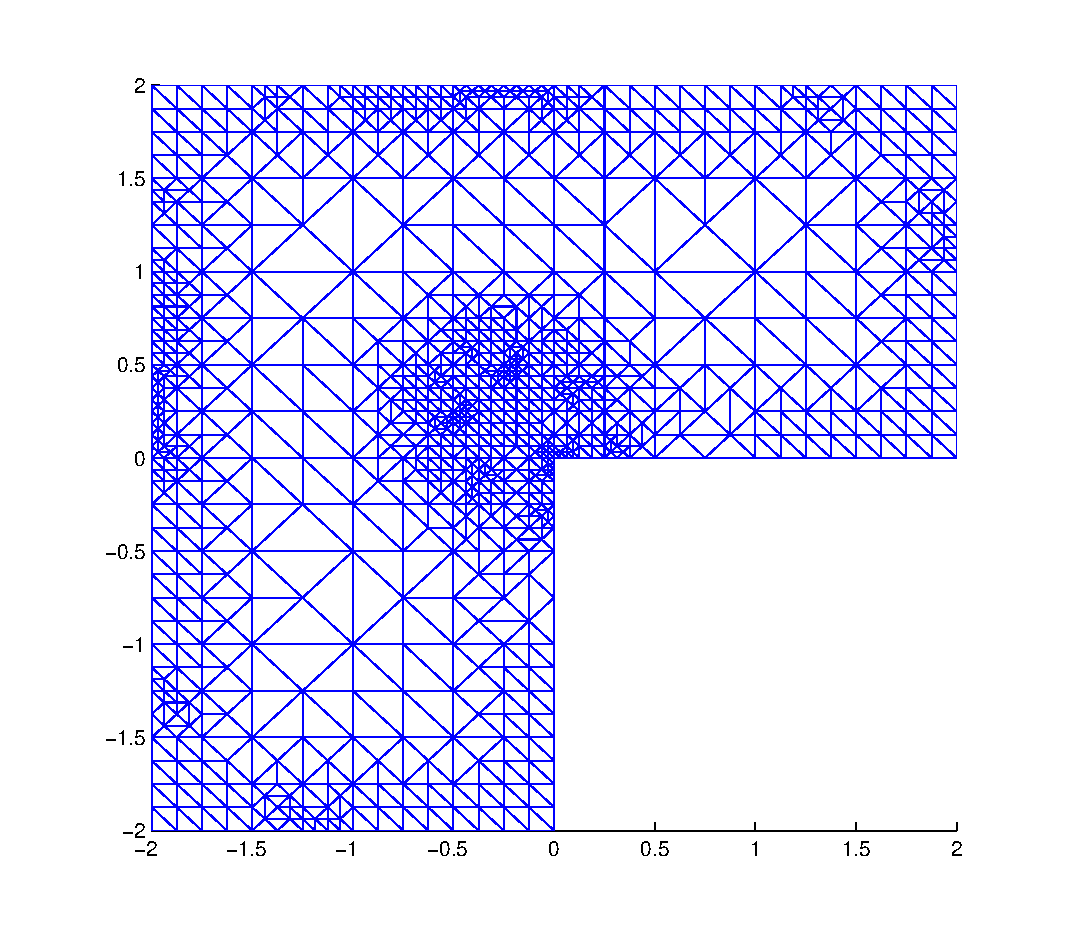
\includegraphics[width=6.26cm]{Abbildungen/mesh_rec6_bsp3.eps}}
\hfill
\subfigure[Verfeinerungsstufe 8]{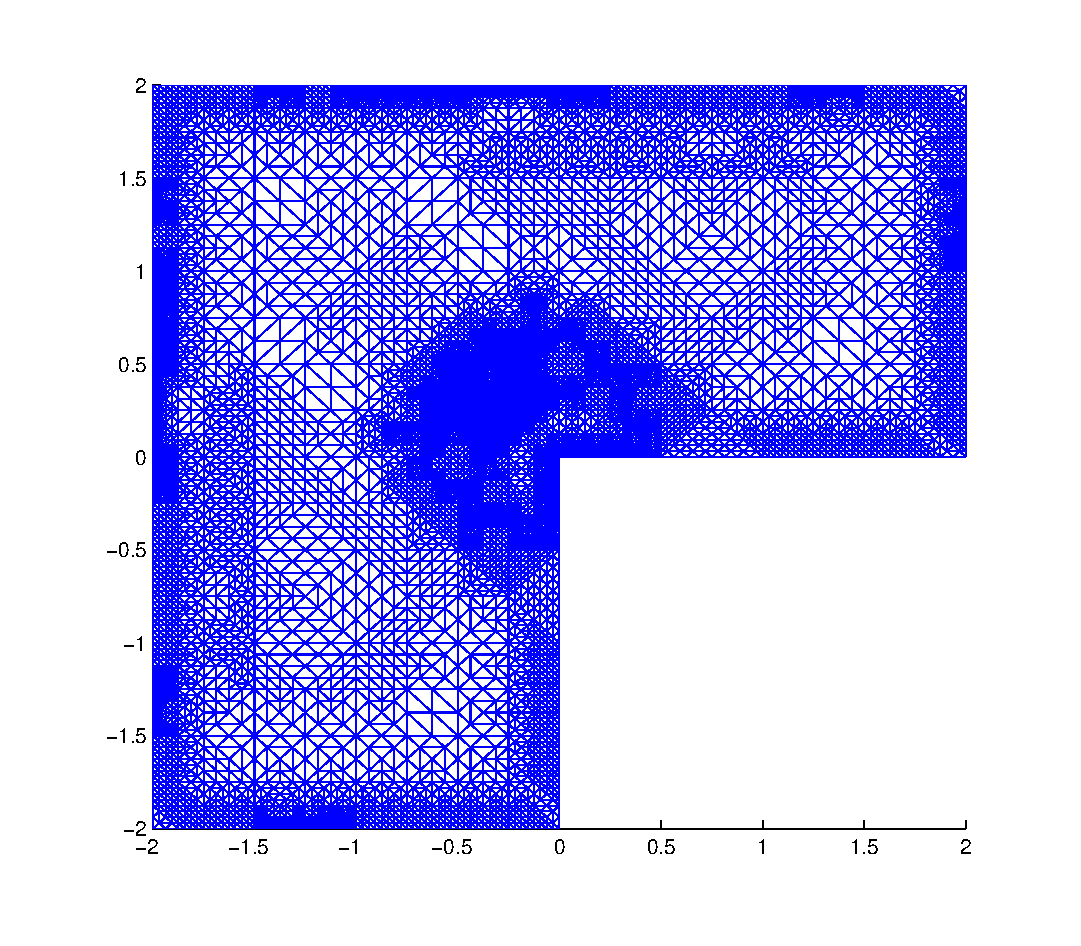
\includegraphics[width=6.26cm]{Abbildungen/mesh_rec8_bsp3.eps}}
\end{center}
\caption{Netzverfeinerungen für das Beispiel \ref{bsp:6.3} mit $\theta_1=\theta_2=0,3$\label{abb:6.8}}
\end{figure}

\begin{figure}[ht]
\begin{center}
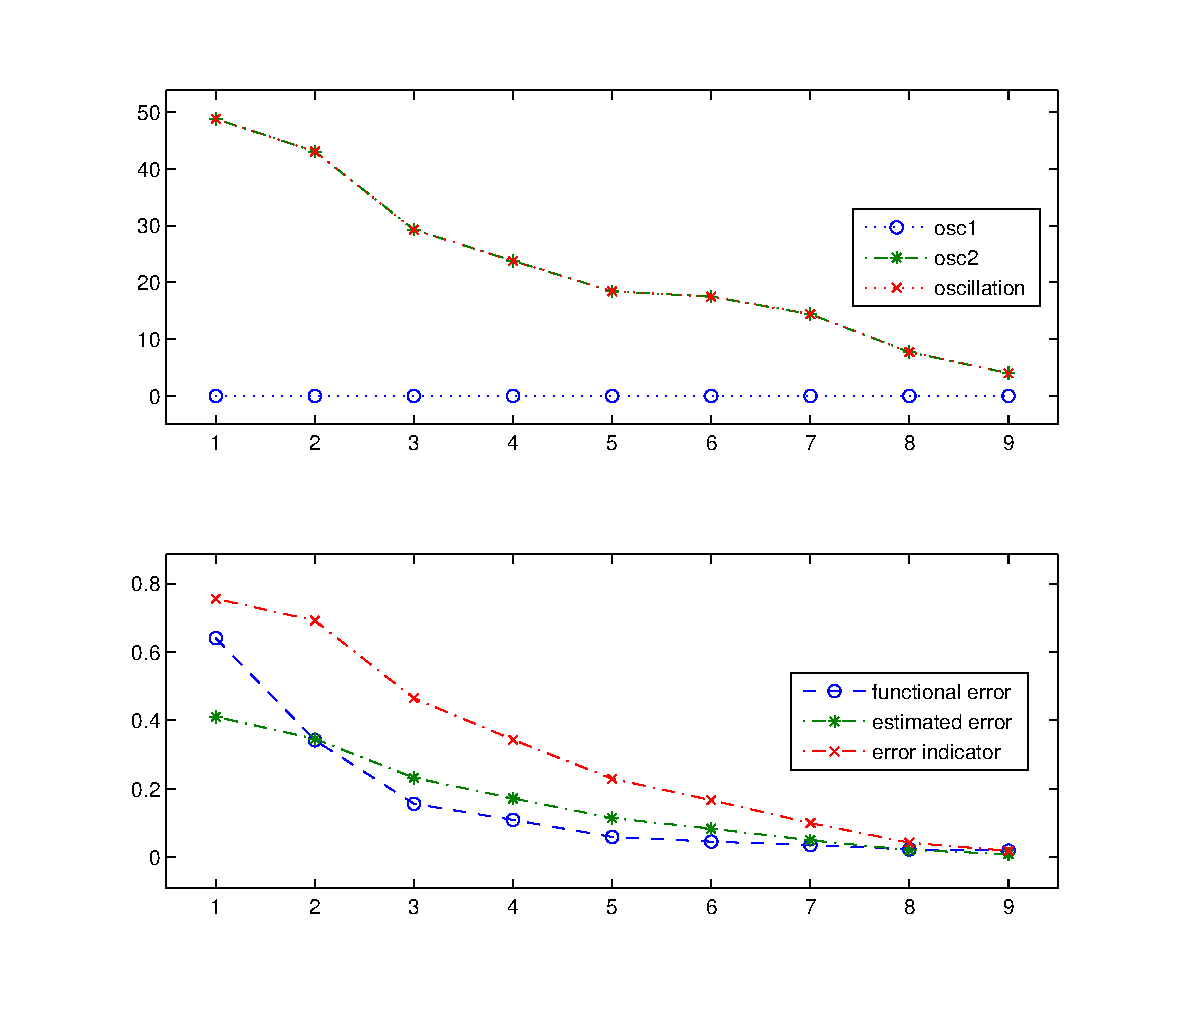
\includegraphics[width=12cm]{Abbildungen/adaptive_solution_example3.eps}
\end{center}
\caption[Diagramm mit dem Fehler und der Oszillation für Beispiel \ref{bsp:6.3}]{Fehlerindikator $\rho_{\mcal S}$, Fehlerschätzer $-\mcal I_{\mcal Q}$ und exakten Fehler $-\mcal I(e)$ für Beispiel \ref{bsp:6.3} mit $\theta_1=0,3$ und $\theta_2=0,3$\label{abb:6.9}}
\end{figure}

\begin{table}[h]
\centering
\begin{tabular}[c]{|c|c|c|c|c|c|c|c|}
	\hline
	 & \multicolumn{4}{c|}{Adaptive Verfeinerung} & \multicolumn{2}{c|}{Uniforme Verfeinerung} \\
	\hline
	Stufe & $\abs{\mcal N}$ & $\rho_{\mcal S}(\eps_{\mcal V})$ & $-\mcal I_{\mcal Q} (\eps_{\mcal V})$ & $-\mcal I(e)$ & $\abs{\mcal N}$ & $-\mcal I (e)$ \\
	\hline
	 1 &  65   &  0.7565 & 0.4109 & 0.6409 & 65 & 0.6409 \\
	 2 &  97 & 0.6922 &0.3464  & 0.3423 & 225 & 0.2826 \\
	 3 & 196  & 0.4652 &  0.2327& 0.1566 & 833 &0.0858  \\
	 4 & 293  & 0.3439 &0.1721 & 0.1094 & 3201 & 0.0333  \\
	 5 &518  & 0.2297 & 0.1150 &  0.0597 &  12545 & 0.0192 \\
	 6 &  717 & 0.1672 & 0.0837 &  0.0460& 49665 &  ––––––– \\
	 7 & 1362 & 0.0999 &0.0500  & 0.0354 & &  \\
	 8 & 5237 & 0.0426 & 0.0213 & 0.0229 &  &  \\
	 9 & 20529 &  0.0189 &0.0095  & 0.0192 & & \\
	\hline
\end{tabular}
\caption[Vergleich von adaptiver und uniformer Verfeinerung für Beispiel \ref{bsp:6.3}]{\label{tab:6.3}Vergleich von adaptiver ($\theta_1=\theta_2=0,3$) und uniformer Verfeinerung für Beispiel \ref{bsp:6.3} mit Angabe des Freiheitsgrades, a posteriori Fehlerschätzer und exaktem Fehler}
\end{table}
\end{bsp}
    
       
\clearpage

\section{Numerisches Beispiel zum Kontaktproblem}
\label{kap:6.2}



\begin{bsp}[\idx{Hertz'sches Kontaktproblem}]\label{bsp:6.4}
Beim Hertz'schen Kontaktproblem betrachten wir einen Zylinder, der auf eine Ebene gepresst wird (vgl. Abbildung \ref{abb:6.10}). Da die Höhe des Zylinders viel größer als der Durchmesser ($d=2$) angenommen werden kann, können wir hier das Prinzip des ebenen Verzerrungszustandes (vgl. Kapitel \ref{kap:2.5.3}) anwenden. 

\begin{figure}[ht]
\begin{center}
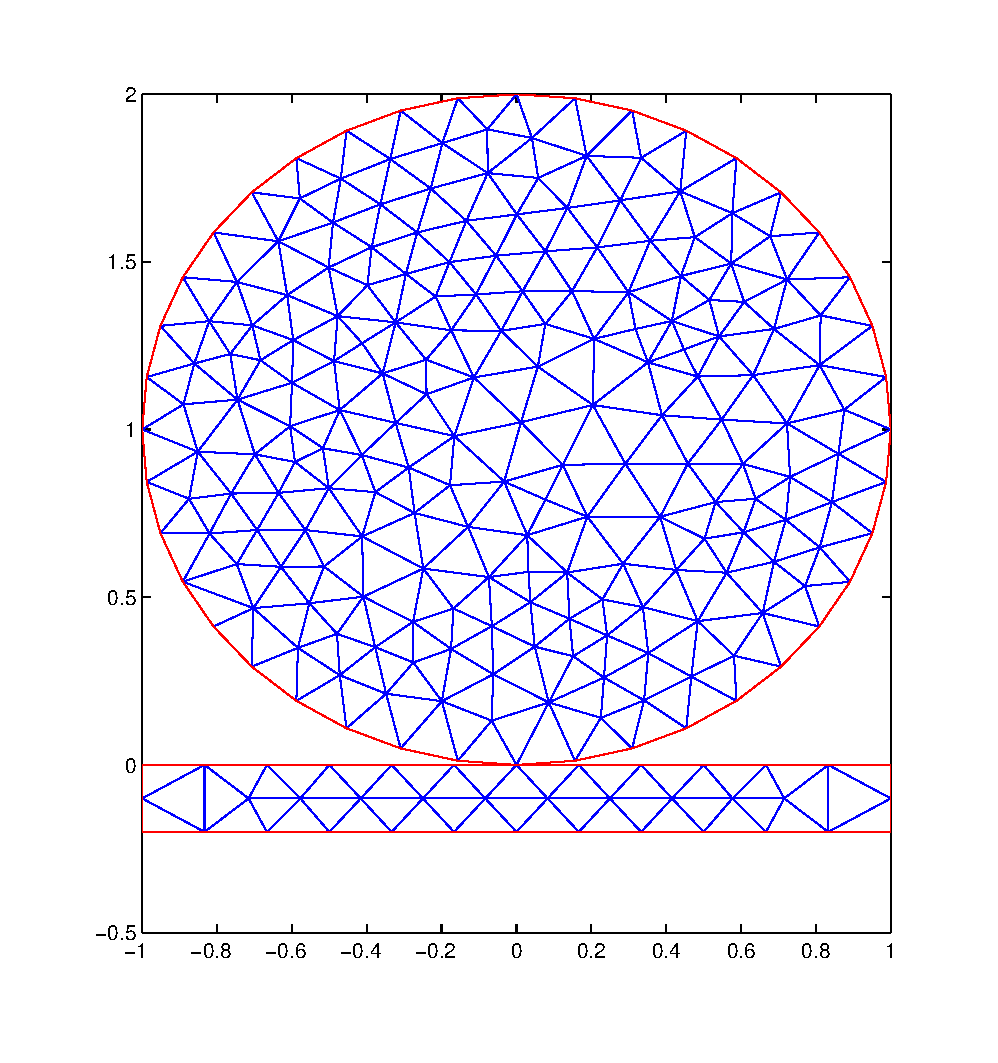
\includegraphics[width=11cm]{Abbildungen/example_4_0,4_depth_6/initial_mesh.eps}
\end{center}
\caption[Darstellung von Beispiel \ref{bsp:6.4} (\idx{Hertz'sches Kontaktproblem})]{Initiales Gitter für das Hertz'sche Kontaktproblem mit $h_{\text{max}} = 0,17$\label{abb:6.10}}
\end{figure}

Wir untersuchen dieses Beispiel (vgl. \cite{CarWri} Beispiel 8.1) für einen Zylinder mit Elastizitätsmodul $E = 7000$ und Poissonzahl $\nu = 0,3$. Die Ebene soll steifer sein, d.h. sie hat das Elastizitätsmodul $E = 10^6$ und die Poissonzahl $\nu = 0,45$. Damit lassen sich die \idx{Lamé-Konstanten} $\lambda$ und $\mu$  für die verschiedenen Teilmengen des Gebietes berechnen und wir können mit dem \idx{Hooke'sche Gesetz} \eqref{eq:2.33} den Zusammenhang zwischen Spannung $\bs \sigma$ und Verzerrung $\bs \eps$ berechnen. Weiter sei der Zylinder mit einer Punktladung $F=100$ am obersten Punkt belastet. Damit jedoch am oberen Rand keine Singularität entsteht, verteilt man die Punktladung auf mehrere Knoten am Rand.

Dies führt zu der Problematik, dass die lokale Aufteilung \eqref{eq:4.92} von $\rho_{\mscr S}$ für die einzelnen Knotenbelastungen nicht angewendet werden kann. Damit gilt
\[
	\rho_{\mscr S} (\bs \eps_{\mscr V}) \not = \sum_{p\in \mcal N} \rho_p (\bs \eps_{\mscr V}) \, .
\]
Dennoch kann man an den Ergebnissen aus Tabelle \ref{tab:6.4} erkennen, dass der Algorithmus \ref{alg:4.1} auch auf das Hertz'sche Kontaktproblem übertragbar ist. Dies ist darin begründet, dass in jedem Verfeinerungsschritt immer derselbe Faktor (abhängig von dem Wert des Fehlerindikators) zwischen der linken und rechten Seite fehlt.

Da der exakte Fehler nicht bekannt ist, berechnen wir ihn hier auch mittels eines feinen Gitters und erhalten
\[
	J(\bs u) \approx -2,29 \, .
\]
An den Ergebnissen aus Tabelle \ref{tab:6.4} bzw. Abbildung \ref{abb:6.11} kann man die Verringerung des Fehlers grundlegend in jedem Verfeinerungsschritt erkennen. Nur im ersten Schritt steigt zunächst der Fehler leicht an, was daran liegen kann, dass sich die Oszillationen in jenem Verfeinerungsschritt nicht verringern. Daher wäre es sinnvoll, den Code noch um die Oszillationsterme zu erweitern. Man kann auch deutlich erkennen, dass die adaptive Verfeinerung mit dem Parameter $\theta = 0,35$ einen geringeren Anstieg des Freiheitsgrades in jedem Verfeinerungsschritt aufweist als die uniforme Verfeinerung.

Für das Hertz'sche Kontaktproblem kann es sinnvoll sein, als Vergleichsparameter für die Genauigkeit der Lösung nicht den Wert des Energiefunktionals zu nehmen, sondern den Wert der Normalenspannung in der Kontaktfläche, da dieser sich exakt  (vgl. \cite{WriggersContact}, Kapitel 14.6.1) berechnen lässt durch
\[
	p_{\text{max}} = \sqrt{\frac F{\pi r} \frac E{(1+\nu)(1-\nu)}} \, .
\]
Diesbezüglich wäre es auch interessant, den Spannungsverlauf innerhalb des Zylinders zu betrachten. Dieser sollte sich achsensymmetrisch zur $y$-Achse entwickeln, wenn auch das erzeugte Gitter nahezu symmetrisch zur $y$-Achse liegt. Dieser Sachverhalt kann ausblickend noch implementiert werden.

%\begin{table}[h]
%\centering
%\begin{tabular}[c]{|c|c|c|c|c|c|c|c|}
%	\hline
%	 & \multicolumn{4}{c|}{Adaptive Verfeinerung} & \multicolumn{2}{c|}{Uniforme Verfeinerung} \\
%	\hline
%	Stufe & $\abs{\mcal N}$ & $\rho_{\mscr S}(\bs \eps_{\mscr V})$ & $-\mscr I_{\mscr Q} (\bs\eps_{\mscr V})$ & $-\mscr I(\bs e)$ & $\abs{\mcal N}$ & $-\mscr I (\bs e)$ \\
%	\hline
%	 1 &  243   &  0.6085 & 0.3042 & 0.1281 &243 & 0.1281 \\
%	 2 &  289 & 0.4030 &0.2015  & 0.2068 & 901 & 0.1414  \\
%	 3 & 370  & 0.2291 &  0.1162& 0.1369 & 3465 & 0.1011 \\
%	 4 & 699  & 0.1068 &0.0542 & 0.0779 &13585 & 0.0790  \\
%	 5 &2682  & 0.0424 & 0.0213 &  0.0333  & & \\
%	 6 & 10503  & 0.0166 & 0.0083 &  0.0107 & & \\
%	\hline
%\end{tabular}
%\caption[Vergleich von adaptiver ($\theta=0,4$) und uniformer Verfeinerung für Beispiel \ref{bsp:6.4}]{\label{tab:6.4}Vergleich von adaptiver und uniformer Verfeinerung für Beispiel \ref{bsp:6.4} mit Angabe des Freiheitsgrades, a posteriori Fehlerschätzer und exaktem Fehler}
%\end{table}

\begin{table}[h]
\centering
\begin{tabular}[c]{|c|c|c|c|c|c|c|c|}
	\hline
	 & \multicolumn{4}{c|}{Adaptive Verfeinerung} & \multicolumn{2}{c|}{Uniforme Verfeinerung} \\
	\hline
	Stufe & $\abs{\mcal N}$ & $\rho_{\mscr S}(\bs \eps_{\mscr V})$ & $-\mscr I_{\mscr Q} (\bs\eps_{\mscr V})$ & $-\mscr I(\bs e)$ & $\abs{\mcal N}$ & $-\mscr I (\bs e)$ \\
	\hline
	 1 &  243   &  0.6085 & 0.3042 & 0.0681 &243 & 0.0681 \\
	 2 &  286 & 0.4091 &0.2045  & 0.1522 & 901 & 0.0814  \\
	 3 & 355  & 0.2567 &  0.1301& 0.1221 & 3465 & 0.0411 \\
	 4 & 594  & 0.1277 &0.0646 & 0.0802 &13585 & 0.0190  \\
	 5 &2266  & 0.0509 & 0.0256 &  0.0396  & & \\
	 6 & 6644  & 0.0205 & 0.0103 &  0.0185 & & \\
	 7 & 26249 & 0.0082 & 0.0041 &  0.0066 &  & \\
	\hline
\end{tabular}
\caption[Vergleich von adaptiver und uniformer Verfeinerung für Beispiel \ref{bsp:6.4}]{\label{tab:6.4}Vergleich von adaptiver ($\theta = 0,35$) und uniformer Verfeinerung für Beispiel \ref{bsp:6.4} mit Angabe des Freiheitsgrades, a posteriori Fehlerschätzer und exaktem Fehler}
\end{table}
    
    

\begin{figure}[ht]
\begin{center}
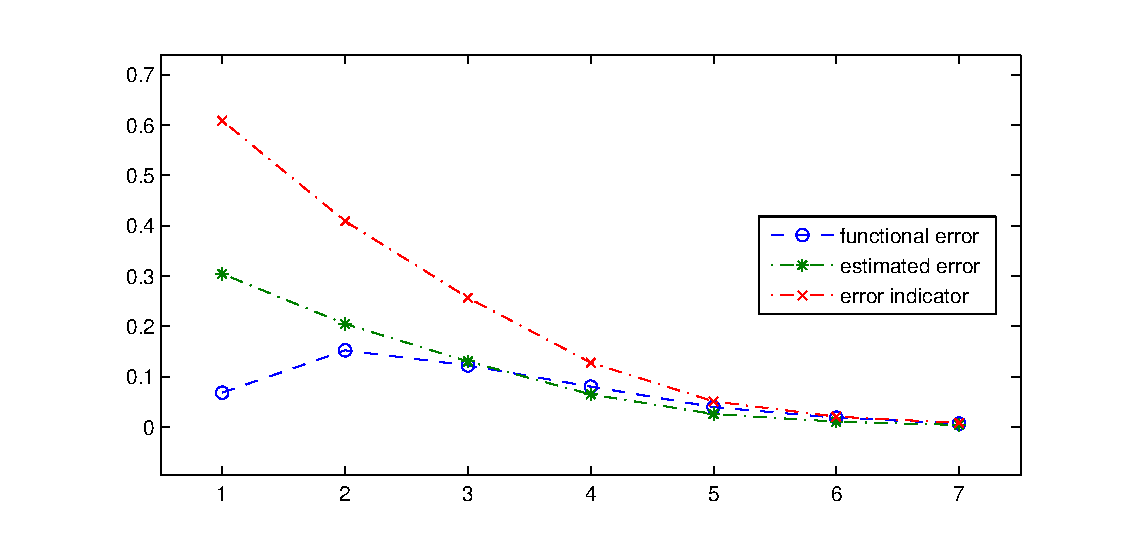
\includegraphics[width=12cm]{Abbildungen/example_4_0,35_depth_6/diagramm.eps}
\end{center}
\caption[Diagramm mit dem Fehler für Beispiel \ref{bsp:6.4}]{Fehlerindikator $\rho_{\mscr S}$, Fehlerschätzer $-\mscr I_{\mscr Q}$ und exakten Fehler $-\mscr I(\bs e)$ für Beispiel \ref{bsp:6.4} mit $\theta=0,35$\label{abb:6.11}}
\end{figure}

In der Abbildung \ref{abb:6.12} sind verschiedene adaptiv erzeugte Gitter zum Parameter $\theta = 0,35$ abgebildet und in Abbildung \ref{abb:6.13} können wir die $x$- und $y$-Komponente des Verschiebungsfeldes $\bs u_{\mscr S}$ einsehen. Hier ist zu erkennen, dass der Zylinder sich erwartungsgemäß durch die Stauchung in $y$-Richtung in $x$-Richtung ausdehnt.

Es ist sinnvoll zu erwähnen, dass die vorliegend implementierte \idx{Gap-Funktion} stückweise linear ist, auch wenn der Zylinder krummlinig ist. Damit ist dieses Beispiel auch konform zu den im Kapitel \ref{kap:4} hergeleiteten Ergebnissen. Die stückweise Lineararität ist darin begründet, dass die Gap-Funktion nur punktweise am Rand des Zylinders ausgewertet wird und der Körper, der mit dem Zylinder in Kontakt steht, eben ist.

\begin{figure}[h]
\begin{center}
\subfigure[Verfeinerungsstufe 3]{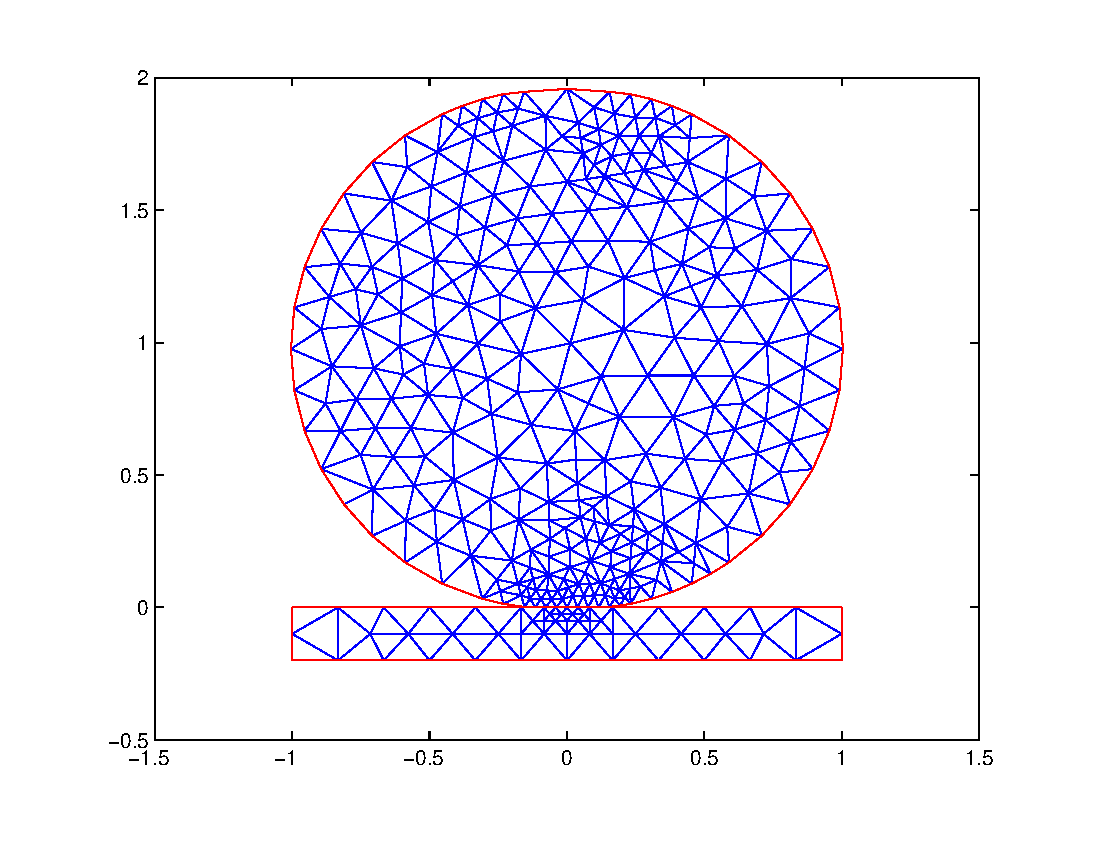
\includegraphics[width=6.26cm]{Abbildungen/example_4_0,35_depth_6/solution_rec_3.eps}}
\subfigure[Verfeinerungsstufe 4]{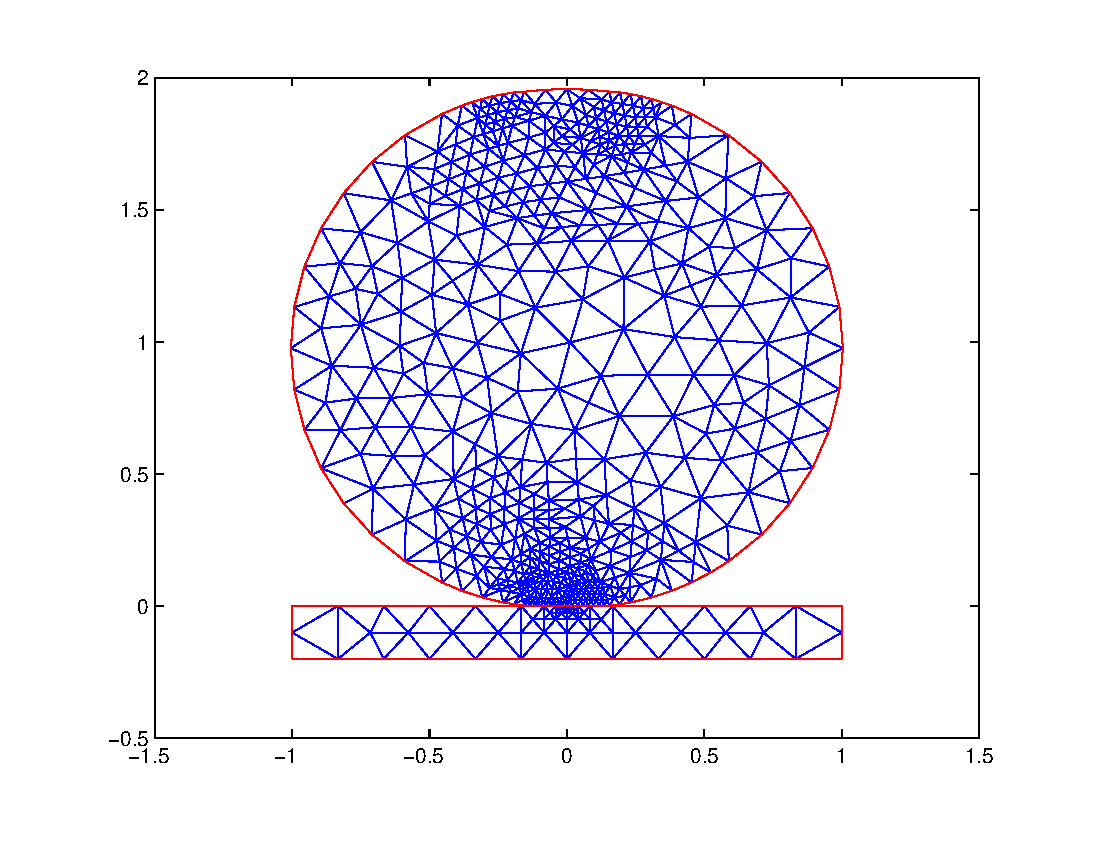
\includegraphics[width=6.26cm]{Abbildungen/example_4_0,35_depth_6/solution_rec_4.eps}}
\subfigure[Verfeinerungsstufe 5]{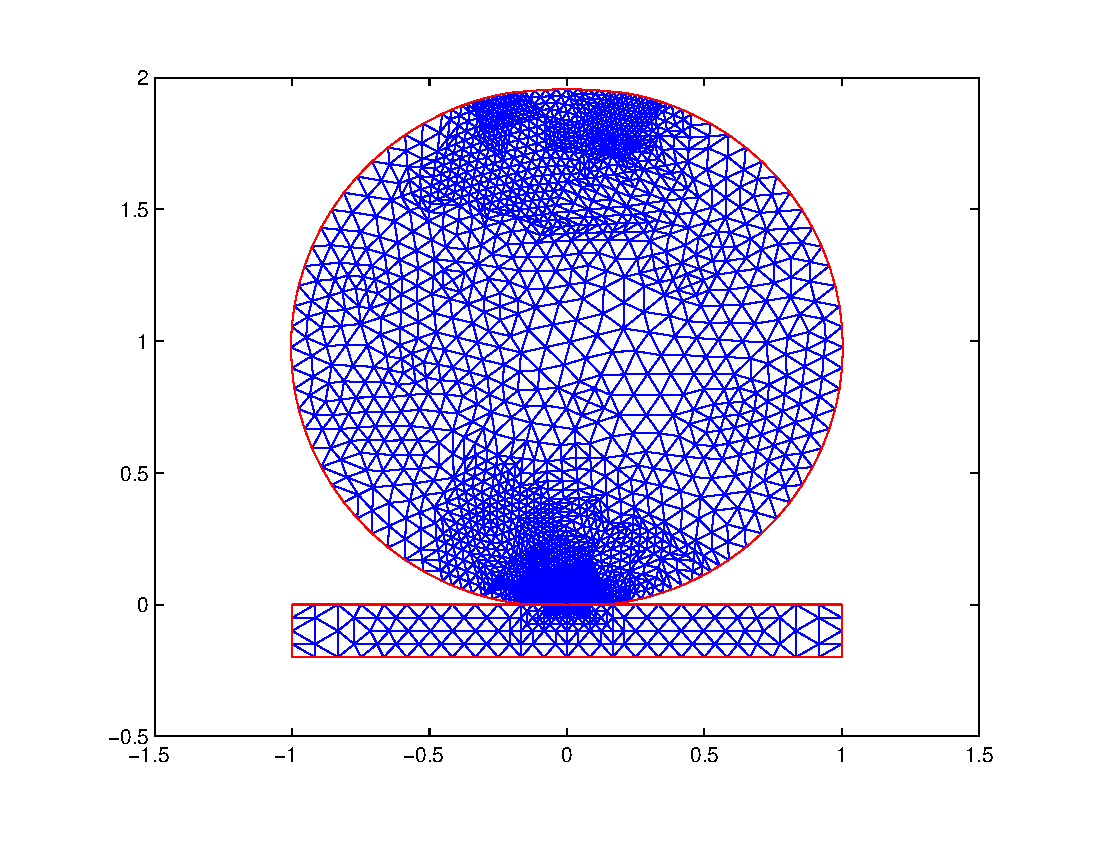
\includegraphics[width=6.26cm]{Abbildungen/example_4_0,35_depth_6/solution_rec_5.eps}}
\subfigure[Verfeinerungsstufe 6]{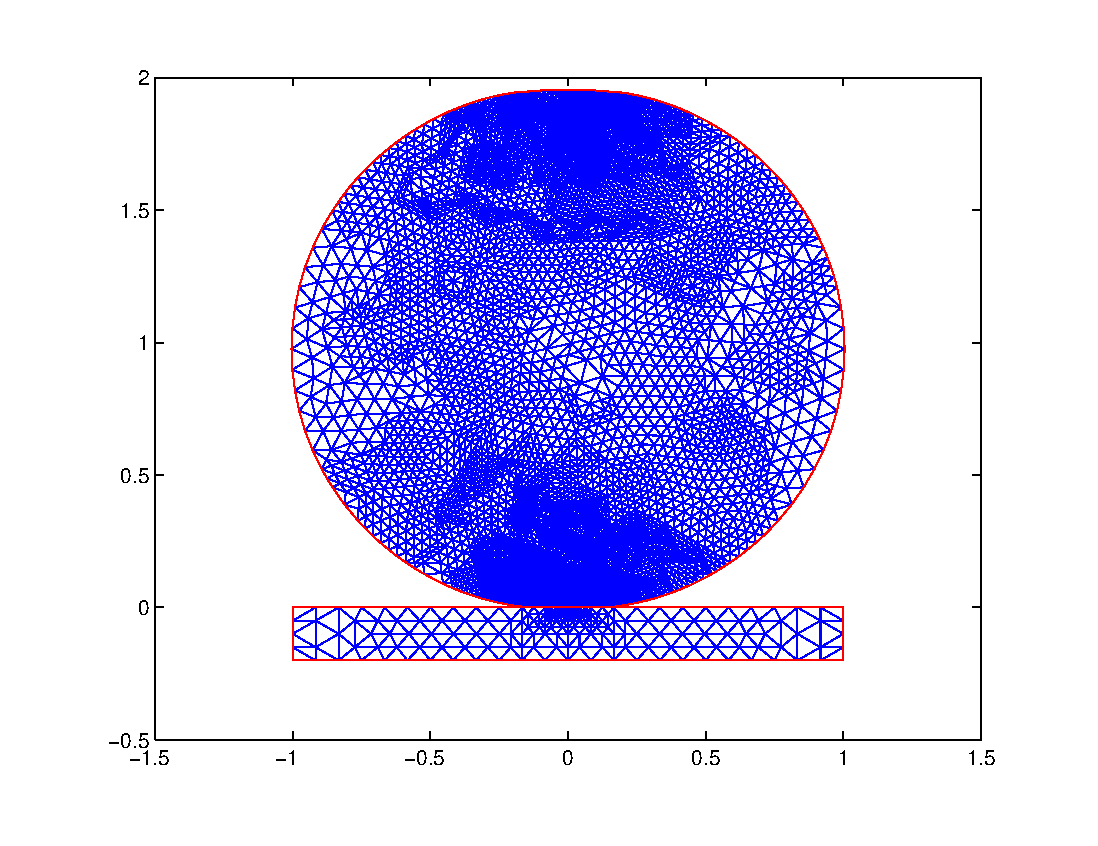
\includegraphics[width=6.26cm]{Abbildungen/example_4_0,35_depth_6/solution_rec_6.eps}}
\end{center}
\caption{Netzverfeinerungen für das Beispiel \ref{bsp:6.4} mit $\theta=0,35$\label{abb:6.12}}
\end{figure}

\begin{figure}[h]
\begin{center}
\subfigure[$x$-Verschiebung]{\includegraphics[width=6.26cm]{Abbildungen/example_4_0,35_depth_6/solution_x_rec_7.eps}}
\hfill
\subfigure[$y$-Verschiebung]{\includegraphics[width=6.26cm]{Abbildungen/example_4_0,35_depth_6/solution_y_rec_7.eps}}
\end{center}
\caption{Abbildung der $x$- und $y$-Komponenten des Verschiebungsfeldes von Beispiel \ref{bsp:6.4} mit $\theta=0,35$\label{abb:6.13}}
\end{figure}

\end{bsp}
   
   
   
   
   
          
   
\newpage

%%% Local Variables: 
%%% mode: latex
%%% TeX-master: "Skript"
%%% End: 
